\documentclass{standalone}

\usepackage{tikz}
\usetikzlibrary{automata,arrows}
\usepackage[compat=1.1.0]{tikz-feynman}
\usepackage{xcolor}

\begin{document}
    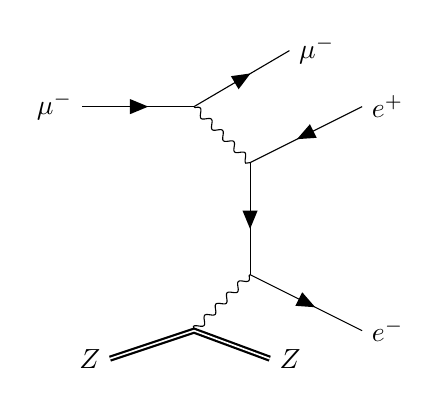
\begin{tikzpicture}
        % Sizes
        \pgfmathsetmacro{\len}{0.05cm}
        \pgfmathsetmacro{\halflen}{\len/4}
        \pgfmathsetmacro{\vertexsize}{\len/20}
        \begin{feynman}
            % vertices
            \vertex (a) at (0, 0);
            \vertex (b) at (0, -1*\len);
            \vertex (d) at (-0.5*\len, 0.5*\len);
            \vertex (c) at (-0.5*\len, -1.5*\len);
            \vertex (i1) at (-1.5*\len, 0.5*\len);
            \vertex (i2) at (0, 1.5*\len);
            \vertex (f1) at (\len, 0.5*\len);
            \vertex (f2) at (\len, -1.5*\len);
            \vertex (f3) at (0.5, 1*\len);
            \vertex (z1) at (-1.25*\len, -1.75*\len);
            \vertex (z2) at (0.25, -1.75*\len);

            % draw diagram
            \diagram* {
                (i1) -- [fermion] (d) -- [fermion] (f3),
                (d) -- [boson] (a),
                (f1) -- [fermion] (a),
                (a) -- [fermion] (b),
                (b) -- [fermion] (f2),
                (b) -- [boson] (c),
            };
            \draw[thick, double] (z1) -- (c) -- (z2);

            % labels
            \node[left] at (i1) {$\mu^-$};
            \node[right] at (f3) {$\mu^-$};
            \node[right] at (f1) {$e^+$};
            \node[right] at (f2) {$e^-$};
            \node[left] at (z1) {$Z$};
            \node[right] at (z2) {$Z$};
        \end{feynman}
    \end{tikzpicture}
\end{document}
